
\documentclass[hyperref={pdfpagelabels=false},ngerman]{beamer}

% stop font warning
\let\Tiny=\tiny
\providecommand\thispdfpagelabel[1]{}

\usepackage[english]{babel}
\usepackage{lmodern}
\usepackage[T1]{fontenc}
\usepackage[utf8]{inputenc}
\usepackage{graphicx,import}
\usepackage{feynmp}
\DeclareGraphicsRule{*}{mps}{*}{} 
\DeclareGraphicsExtensions{.pdf}
\usepackage{amsmath,amssymb,amstext,amsfonts} % mathrsfs
\usepackage{array,booktabs,tabularx}
\usepackage{tikz,tikz-uml,pgf-pie}
\usetikzlibrary{shapes,calc,arrows,positioning}
\tikzstyle{block} = [rectangle, draw, text width=7em, text centered, minimum height=2em]
\tikzstyle{arrow} = [draw, -latex, thick]
\tikzstyle{arrow2} = [draw, latex-latex, thick]
\tikzstyle{quark}  = [rectangle, draw, fill=yellow, minimum width=2em, text centered, minimum height=2em]
\tikzstyle{lepton} = [rectangle, draw, fill=red!50, minimum width=2em, text centered, minimum height=2em]
\tikzstyle{gauge}  = [circle   , draw, fill=green , minimum size=2em, inner sep=0pt, text centered]
\tikzstyle{scalar} = [diamond  , draw, fill=blue!40, minimum width=2.3em, text centered, minimum height=2.3em, inner sep=0pt]
\tikzstyle{goldstone} = [diamond, draw, dashed, fill=blue!30, minimum width=2.3em, text centered, minimum height=2.3em, inner sep=0pt]
\tikzstyle{squark}   = [diamond, draw, fill=yellow, minimum width=2.3em, text centered, minimum height=2.3em, inner sep=0pt]
\tikzstyle{slepton}  = [diamond, draw, fill=red!50, minimum width=2.3em, text centered, minimum height=2.3em, inner sep=0pt]
\tikzstyle{gaugino}  = [rectangle, draw, fill=green , minimum size=2em, inner sep=0pt, text centered]
\tikzstyle{higgsino} = [rectangle, draw, fill=blue!40  , minimum width=2em, text centered, minimum height=2em]
\tikzstyle{inert}    = [diamond  , draw, fill=teal!80, minimum width=2.3em, text centered, minimum height=2.3em, inner sep=0pt]
\tikzstyle{inertino} = [rectangle, draw, fill=teal!80, minimum width=2em, text centered, minimum height=2em]
\tikzstyle{phantom}  = [rectangle, minimum width=2em, text centered, minimum height=2em]
\usepackage{slashed}
\usepackage{fixltx2e} % textsubscript
\usepackage{multirow}
\usepackage{tcolorbox}
\usepackage{pifont}
\usepackage{xspace}
\usepackage{hyperref}
\hypersetup{colorlinks,linkcolor=,urlcolor=blue}
\usepackage{listings}
\lstset{breaklines=true,
  breakatwhitespace=true,
%  numbers=left,
  numberstyle=\tiny,
  stepnumber=1,
  basicstyle=\ttfamily\footnotesize,
  commentstyle=\ttfamily\color{gray},
  postbreak={\mbox{{$\hookrightarrow$}}\space\space},
  breakindent=10pt,
  breakautoindent=false,
  showspaces=false,
  showstringspaces=false,
  frame=single}

\definecolor{darkgreen}{RGB}{0,176,0}

\newcommand{\cmark}{\ding{51}}%
\newcommand{\xmark}{\ding{55}}%
\newcommand{\fmfvcenter}[1]{\;\vcenter{\hbox{\fmfreuse{#1}}}\;}
\newcommand{\eh}[1]{\,\mathsf{#1}}
\newcommand{\GeV}{\eh{GeV}}
\newcommand{\TeV}{\eh{TeV}}
\newcommand{\ok}{\textcolor{darkgreen}{\cmark}}
\newcommand{\notok}{\textcolor{red}{\xmark}}
\newcommand{\maybe}{\textcolor{gray}{\cmark}}
\newcommand{\meh}{\textcolor{gray}{\textbf{\huge\lower.1em\hbox{-}}}}
\newcommand{\Lagr}{\mathcal{L}}
\newcommand{\MS}{\ensuremath{M_S}}
\newcommand{\mathi}{\mathsf{i}}
\newcommand{\mycite}[1]{\ensuremath{\text{\textcolor{darkgray}{\tiny [#1]}}}}
\newcommand{\bigcite}[1]{\textcolor{darkgray}{[#1]}}
\newcommand{\dimrep}[1]{\mathbf{#1}}
\newcommand{\dimrepadj}[1]{\mathbf{\overline{#1}}}
\newcommand{\ESSM}{E\textsubscript{6}SSM}
\newcommand{\CESSM}{CE\textsubscript{6}SSM}
\DeclareMathOperator{\tildeRe}{\widetilde Re}
\DeclareMathOperator{\sign}{sign}
\DeclareMathOperator{\re}{Re}
\DeclareMathOperator{\im}{Im}
\renewcommand{\emph}{\textbf}
\newcommand{\dd}{\mathsf{d}}
\newcommand{\myurl}[1]{\href{#1}{#1}}
\newcommand{\Superpot}{\mathcal{W}}
\newcommand{\SuperField}[1]{#1}
\newcommand{\ConjSuperField}[1]{\bar{#1}}
\newcommand{\UY}{\ensuremath{U(1)_{Y}}}
\newcommand{\UN}{\ensuremath{U(1)_{N}}}
\newcommand{\Uem}{\ensuremath{U(1)_\text{em}}}
\newcommand{\SUL}{\ensuremath{SU(2)_\text{L}}}
\newcommand{\SUc}{\ensuremath{SU(3)_\text{c}}}
\newcommand{\SOten}{\ensuremath{{SO(10)}}}
\newcommand{\comma}{,}
\newcommand{\DRbar}{\ensuremath{\overline{\text{DR}}}}
\newcommand{\MSbar}{\ensuremath{\overline{\text{MS}}}}
\newcommand{\SM}{\ensuremath{\text{SM}}}
\newcommand{\MSSM}{\ensuremath{\text{MSSM}}}
\newcommand{\pole}{\ensuremath{\text{pole}}}
\newcommand{\tree}{\ensuremath{\text{tree}}}
\newcommand{\fsstar}{\textbf{*}}
\newcommand{\fs}{\texttt{FlexibleSUSY}\xspace}
\newcommand{\fsh}{\texttt{FS+H}\xspace}
\newcommand{\feft}{\texttt{FlexibleEFTHiggs}\xspace}
\newcommand{\hssusy}{\texttt{HSSUSY}\xspace}
\newcommand{\Himalaya}{\texttt{Himalaya}\xspace}
\newcommand{\FH}{\texttt{FeynHiggs}\xspace}
\newcommand{\SPheno}{\texttt{SPheno}\xspace}
\newcommand{\SARAH}{\texttt{SARAH}\xspace}
\newcommand{\Zv}{\ensuremath{\backslash\mkern-11.0mu{Z_3}}}
\newcommand{\downrightknickarrow}{\mathrel{\scalebox{1.3}{\rotatebox[origin=c]{180}{$\Lsh$}}}}
\newcommand{\threelinebrace}{$\left. \begin{array}{c} \\ \\ \\ \end{array} \right\rbrace$}
\newcommand{\fivelinebrace}{$\left. \begin{array}{c} \\ \\ \\ \\ \\ \end{array} \right\rbrace$}
\newcommand{\twolinebrace}{$\left. \begin{array}{c} \\ \\ \end{array} \right\rbrace$}
\newcommand{\elevenlinebrace}{$\left. \begin{array}{c} \\ \\ \\ \\ \\ \\ \\ \\ \\ \\ \\ \end{array} \right\rbrace$}
\newcommand{\at}{\alpha_t}
\newcommand{\ab}{\alpha_b}
\newcommand{\atau}{\alpha_\tau}
\newcommand{\as}{\alpha_s}
\newcommand{\avnote}[1]{\textcolor{blue}{[#1]}}

% set look of slides
\usetheme{Madrid}
\useoutertheme{default}
\useinnertheme{circles}
\usecolortheme{default}
\beamertemplatenavigationsymbolsempty % keine Navigationselemente
\setbeamersize{text margin left = 1cm, text margin right = 1cm}

% define footer
\makeatletter
\setbeamertemplate{footline}
{
  \hfill\hbox{\insertframenumber{} / \inserttotalframenumber\hspace*{4pt}}%
  \vskip3pt%
}
\makeatother
\usecolortheme{tud}

\title{KUTS paper -- Chapter 4 Hybrid}

\author[Alexander Voigt]{Henning Bahl, Alexander Voigt}

\date{KUTS-9 Würzburg\\[1em] 16--18/07/2018}

% \institute[Aachen]{RWTH Aachen}
\subject{FlexibleSUSY,MSSM,Higgs,FlexibleEFTHiggs}
\keywords{FlexibleSUSY,MSSM,Higgs,FlexibleEFTHiggs}

%%%%%%%%%%%%%%%%%%%%%%%%%%%%%%%%%%%%%%%%%%%%%%%%%%%%%%%%%%%%%%%%%%%%%%%%%%%%%

\begin{document}

%%%%%%%%%%%%%%%%%%%%%%%%%%%%%%%%%%%%%%%%%%%%%%%%%%%%%%%%%%%%%%%%%%%%%%%%%%%%%

% Savebox which contains the the Feynman rules
\newsavebox{\feynmanrules}
\sbox{\feynmanrules}{
\begin{fmffile}{Feynman/higgs} % file name and path
  \fmfset{thin}{.8pt}
  \fmfset{wiggly_len}{5mm}
  \fmfset{dash_len}{2.5mm}
  \fmfset{dot_size}{1thick}
  \fmfset{arrow_len}{2.5mm}
  \fmfset{curly_len}{2.5mm}

\begin{fmfgraph*}(60,60)
  \fmfkeep{hX}
  \fmfleft{v1}
  \fmfright{v2}
  \fmf{higgs}{v1,c1}
  \fmf{higgs}{c2,v2}
  \fmf{quark,left,tension=0.5,label=$X$}{c1,c2}
  \fmf{quark,left,tension=0.5}{c2,c1}
\end{fmfgraph*}

\begin{fmfgraph*}(60,60)
  \fmfkeep{htop}
  \fmfleft{v1}
  \fmfright{v2}
  \fmf{higgs}{v1,c1}
  \fmf{higgs}{c2,v2}
  \fmf{quark,left,tension=0.5,label=$t$}{c1,c2}
  \fmf{quark,left,tension=0.5}{c2,c1}
\end{fmfgraph*}

\begin{fmfgraph*}(60,60)
  \fmfkeep{hstop}
  \fmfleft{v1}
  \fmfright{v2}
  \fmf{higgs}{v1,c1}
  \fmf{higgs}{c2,v2}
  \fmf{scalar,left,tension=0.5,label=$\tilde{t}_i$}{c1,c2}
  \fmf{scalar,left,tension=0.5}{c2,c1}
\end{fmfgraph*}

\begin{fmfgraph*}(60,60)
  \fmfkeep{hstopA}
  \fmfleft{v1}
  \fmfright{v2}
  \fmf{higgs}{v1,c,v2}
  \fmf{scalar,right,tension=0.8,label=$\tilde{t}_i$}{c,c}
\end{fmfgraph*}

\begin{fmfgraph*}(60,60)
  \fmfkeep{htoptad}
  \fmfleft{v1}
  \fmfright{v2}
  \fmftop{t1}
  \fmf{higgs}{v1,c,v2}
  \fmffreeze
  \fmf{higgs}{c,c1}
  \fmf{quark,right,tension=0.3,label=$t$}{c1,c2}
  \fmf{quark,right,tension=0.3}{c2,c1}
  \fmf{phantom,tension=10}{c2,t1}
\end{fmfgraph*}

\begin{fmfgraph*}(60,60)
  \fmfkeep{hstoptad}
  \fmfleft{v1}
  \fmfright{v2}
  \fmftop{t1}
  \fmf{higgs}{v1,c,v2}
  \fmffreeze
  \fmf{higgs}{c,c1}
  \fmf{scalar,right,tension=0.3,label=$\tilde{t}_i$}{c1,c2}
  \fmf{scalar,right,tension=0.3}{c2,c1}
  \fmf{phantom,tension=10}{c2,t1}
\end{fmfgraph*}
\end{fmffile}
}

%%%%%%%%%%%%%%%%%%%%%%%%%%%%%%%%%%%%%%%%
\begin{frame}[plain]
  \tikz [remember picture,overlay]
  \node at
    ([yshift=1.3cm,xshift=4cm]current page.south)
    {\includegraphics[height=2cm]{images/RWTH_Logo}};
  \titlepage  
\end{frame}

%%%%%%%%%%%%%%%%%%%%%%%%%%%%%%%%%%%%%%%%
\begin{frame}{Contents}
  \tableofcontents
\end{frame}

\section{Motivation}

\begin{frame}{4.1 Motivation}
  \begin{columns}
    \begin{column}{0.5\textwidth}
      \centering
      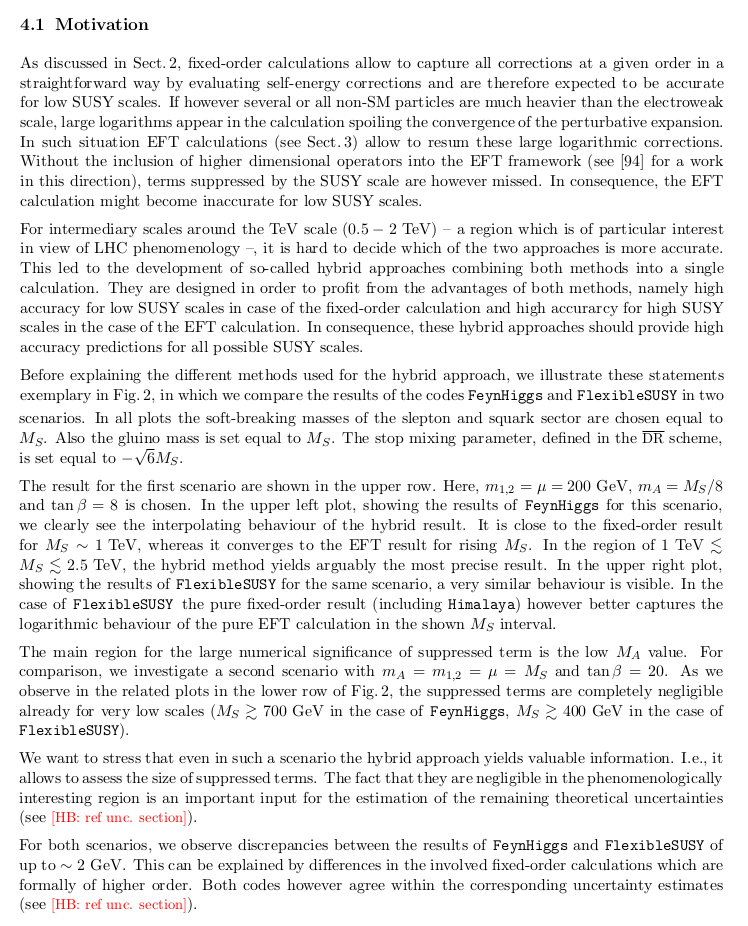
\includegraphics[width=\textwidth]{{{plots/kuts-9/4.1}}}
    \end{column}
    \begin{column}{0.5\textwidth}
      Statements:
      \begin{itemize}
      \item In the currently interesting region $\MS = 0.5$--$1\TeV$ it is
        not clear whether a FO or EFT calculation is more accurate \\
        $\Rightarrow$ use hybrid calculation in that region
      \item Hybrid calculation allows study of suppressed terms \\
        $\Rightarrow$ can conclude when EFT is appropriate
      \end{itemize}
    \end{column}
  \end{columns}
\end{frame}

\begin{frame}{4.1 Motivation}
  Illustration in \FH and \fs:
  \begin{columns}
    \begin{column}{0.6\textwidth}
      \begin{center}
        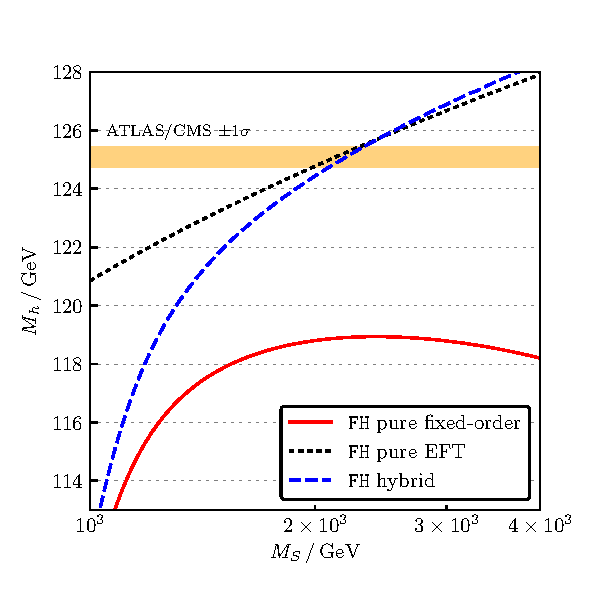
\includegraphics[width=0.49\textwidth]{plots/kuts-9/FH_1}
        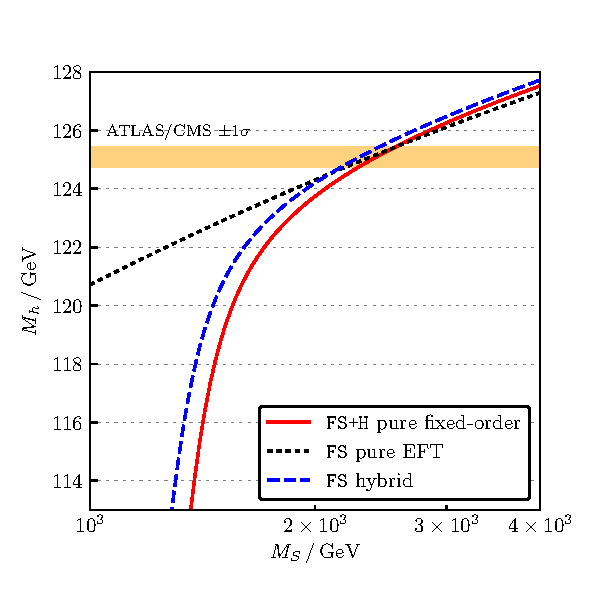
\includegraphics[width=0.49\textwidth]{plots/kuts-9/FS_3L}\\
        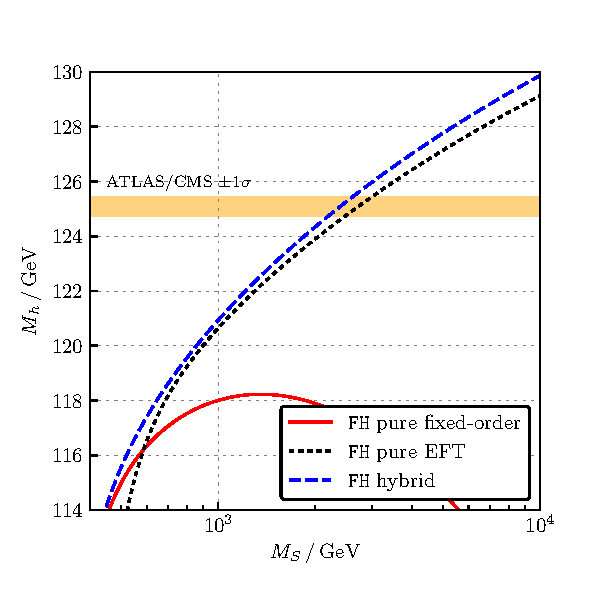
\includegraphics[width=0.49\textwidth]{plots/kuts-9/FH_2}
        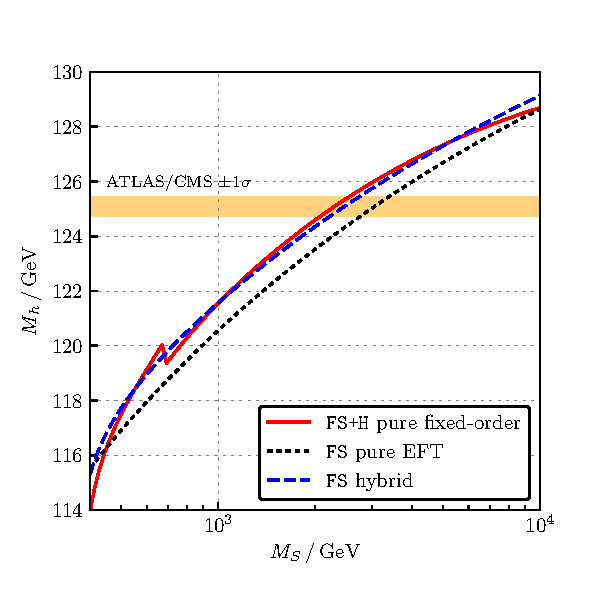
\includegraphics[width=0.49\textwidth]{plots/kuts-9/FS_3L_2}
      \end{center}
    \end{column}
    %
    \begin{column}{0.4\textwidth}
      Top row: $m_A = \MS/8, t_\beta = 8$\\[1em]
      Bottom row: $m_A = \MS, t_\beta = 20$\\[1em]
      Statements:
      \begin{itemize}
      \item Low $m_A$: hybrid interpolates between $1$--$2\TeV$.
        \texttt{FS+H} better captures logarithmic behaviour of EFT
      \item High $m_A$: suppressed terms are negligible for
        $\MS \gtrsim 700\GeV, 400\GeV$
      \end{itemize}
    \end{column}
  \end{columns}
\end{frame}

\section{Methods}

\begin{frame}{4.2 Methods}
    \begin{columns}
    \begin{column}{0.5\textwidth}
      \centering
      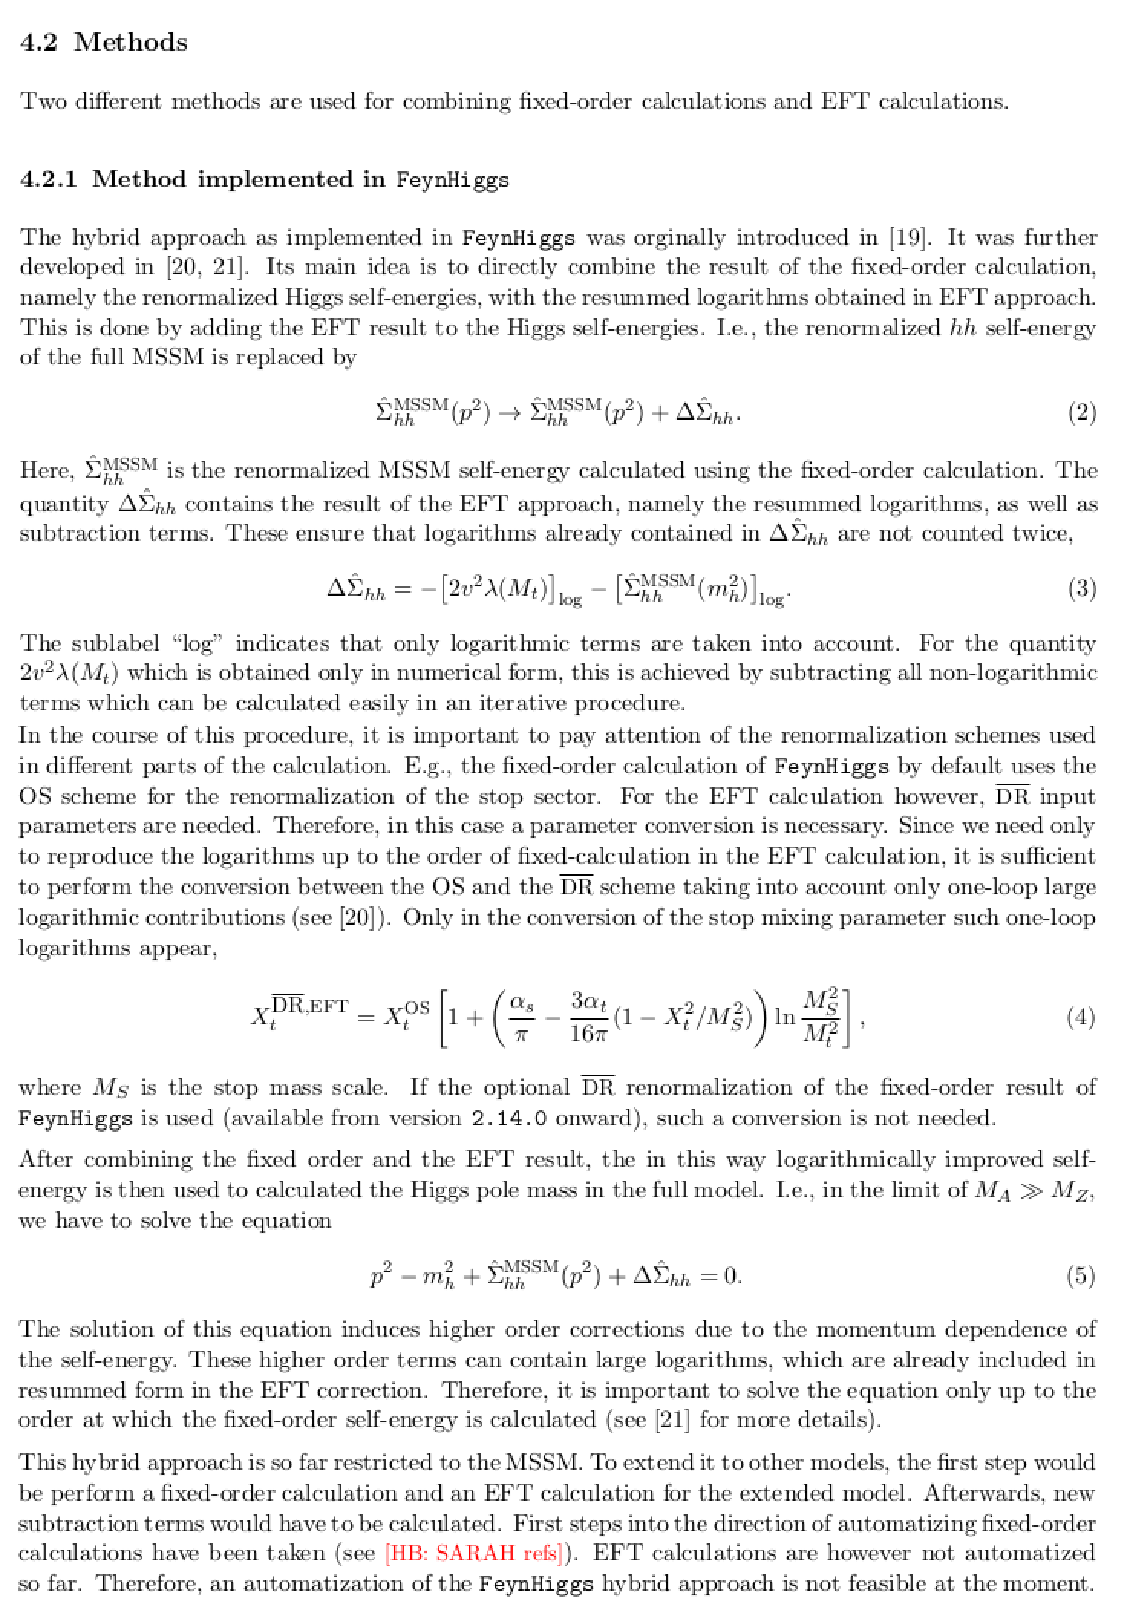
\includegraphics[width=\textwidth]{{{plots/kuts-9/4.2}}}
    \end{column}
    \begin{column}{0.5\textwidth}
      \FH:
      \begin{align*}
        M_h^2 = (M_h^2)_{\text{FO}} - (M_h^2)_{\text{logs}} + (M_h^2)_{\text{res}}
      \end{align*}
      Notes:
      \begin{itemize}
      \item \DRbar\ $\leftrightarrow$ OS conversion
      \item $p^2$ iteration
      \end{itemize}
      Pros/Cons:
      \begin{itemize}
      \item[\ok] 2L accuracy
      \item[\ok] CPV
      \item[\notok] restricted to MSSM
      \end{itemize}
    \end{column}
  \end{columns}
\end{frame}

\begin{frame}{4.2 Methods}
    \begin{columns}
    \begin{column}{0.5\textwidth}
      \centering
      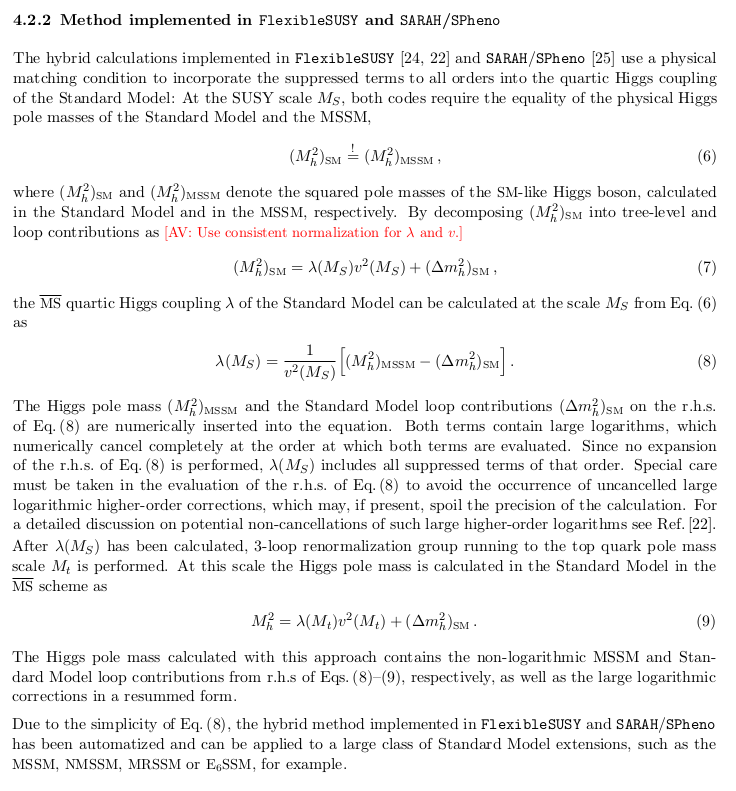
\includegraphics[width=\textwidth]{{{plots/kuts-9/4.2.2}}}
    \end{column}
    \begin{column}{0.5\textwidth}
      \fs (\feft) and \SARAH/\SPheno:
      \begin{align*}
        (M_h^2)_{\SM} &\overset{!}{=} (M_h^2)_{\MSSM} \text{ at } Q = \MS
      \end{align*}
      Notes:
      \begin{itemize}
      \item care must be taken to avoid large higher order logs
      \end{itemize}
      Pros/Cons:
      \begin{itemize}
      \item[\ok] not restricted to MSSM
      \item[\notok] extension to 2L tricky (work in progress)
      \end{itemize}
    \end{column}
  \end{columns}
\end{frame}

\section{Status}

\newcommand{\al}{\alpha}
\begin{frame}{4.3 Status}
  \begin{table}
    \def\arraystretch{1.3}
    \centering
    \scalebox{0.75}{
    \begin{tabular}{llll}
      \toprule
      & fixed-order                 & \multirow{2}{*}{resummation order} & \multirow{2}{*}{low-energy EFTs}\\
      & (incl. $O(v^2/\MS^2)$)      &                                    &                                 \\
      \midrule
      \FH     & LO+NLO+NNLO$^*$     & LL+NLL+NNLL$^\dagger$               & SM (+ $\chi^{0,\pm}$, $\tilde{g}$),        \\
      &                             &                                    & THDM (+ $\chi^{0,\pm}$, $\tilde{g}$)$^{**}$ \\
      \fs     & LO+NLO              & LL+NLL                             & SM                              \\
      \SARAH/\SPheno & LO+NLO+NNLO$^\ddagger$ & LL                                & SM                              \\
      \bottomrule
    \end{tabular}}
  \end{table}
  $^*$Only contributions of
  $O(\al_s (\al_t + \al_b) + (\al_t + \al_b)^2)$\\
  $^\dagger$Only contributions of $O(\al_s,\al_t)$\\
  $^\ddagger$Only contributions of
  $O(\al_s (\al_t + \al_b) + (\al_t + \al_b)^2 + \al_\tau\al_b +
  \al_\tau^2)$\\
  $^{**}$Not yet publicly available
\end{frame}

\section{Advances during KUTS}

\begin{frame}{4.4 Advances during KUTS}
  \begin{itemize}
  \item \FH:
    \begin{itemize}
    \item EW contributions, gaugino thresholds, NNLL resummation \mycite{1608.01880}
    \item investigation of large differences to other codes \mycite{1706.00346}
    \item refinement of hybrid method \mycite{1706.00346}
  \end{itemize}
  \item \feft:
    \begin{itemize}
    \item implementation of hybrid method \mycite{1609.00371}
    \item improved to NLL accuracy \mycite{1710.03760}
  \end{itemize}
  \item \SARAH/\SPheno:
    \begin{itemize}
    \item implementation of hybrid method \mycite{1703.03267}
    \end{itemize}
  \end{itemize}
\end{frame}

\section{Prospects}

\begin{frame}{4.5 Prospects}
  \begin{itemize}
  \item Advance \feft to NNLO + NNLL
  \item Improvement on theoretical uncertainties
  \item Further low-energy models (not only SM as EFT)
  \item Further high-energy models (not only MSSM as UV theory)
  \end{itemize}
\end{frame}

\end{document}
